\begin{bibunit}[IEEEtran.bst]

\chapter*{Introduction}
\addcontentsline{toc}{chapter}{Introduction}
\chaptermark{Introduction}

Understanding and anticipating the ramifications of climate change represents a pressing challenge of our era.
Enhancing our knowledge of Earth's systems is a key factor in confronting this challenge.
  Given that the primary source of factual information about the Earth system is observational data, improving our ability to exploit these data could lead to better monitoring and understanding of our planet.
  This thesis focus on the development of methods to exploit satellite observations for improving our knowledge of ocean surface dynamics. 
  More specifically we're asking how advances in deep learning research can be beneficial to ocean observation analysis.
  
  In order to introduce the potentials of deep learning for tackling observation problems, we'll introduce the necessary methodological components involved when addressing an observation problem by walking through the development of a thermometer calibration procedure. This simplified problem will help illustrate and contextualize the complementary roles of data and domain knowledge when addressing this class of problem and naturally invite deep learning components in certain aspects of the resolution. 
  
  This will first consist in decomposing the process of mapping the level of the thermometer to the temperature. Then we'll look at the challenges met when evaluating a calibrated thermometer. We'll consider the different sources of errors before finally formalizing the necessary components for developing a thermometer calibration procedure.
%   \section{Summary}
% Understanding and anticipating the ramifications of climate change represents a pressing challenge of our era. Enhancing our knowledge of Earth's systems is a key factor in confronting this challenge.
%   Given that the primary source of factual information about the Earth system is observational data, improving our ability to exploit this data could lead to better monitoring and understanding of our planet.
%   Concurrently, recent advancements in deep learning provide robust tools that continually push performance boundaries across a myriad of tasks. 
%   This situation raises an intriguing question: Can deep learning assist in extracting meaningful insights from Earth observations?
%
% Observing ocean surface dynamics through satellite altimetry offers a compelling case study.
%   Currently, operational products do not resolve processes below 150 km, which are essential for climate monitoring.
%   This situation underscores a significant gap in our observational capabilities.
%   The recent deployment of a novel sensor during the SWOT satellite mission provides numerous opportunities to address this gap.
%   This new sensor introduces unprecedented calibration challenges due to previously unseen errors, but it also promises to enhance the reconstruction of Sea Surface Height (SSH) maps.
%
% Despite the significant potential of deep learning as a generic tool, two critical factors seem to determine progress of its application to a specific domain. The first factor is quality and availability of data, indeed the creation of large, curated datasets, like ImageNet in computer vision or ThePile in natural language processing have shown to dramatically expedite the development of novel approaches. The second factor is the design of informed architectural patterns that are particularly suited to the given problem, leading to performance breakthroughs. Examples of these include convolution techniques in computer vision, attention mechanisms in natural language processing, and U-Net architectures for hierarchical data. These two facets — comprehensive, well-curated datasets and efficient architectural patterns — can greatly advance the field, propelling research and application development in exciting directions.
%
% The transdisciplinary nature of this work also introduces unique challenges. The intricacies of ocean observation data and the criteria for precisely evaluating the estimation of geophysical quantities can represent a considerable barrier for ML scientists. Similarly, the logistical aspects and accumulated best practices required to successfully train and utilize a neural network can deter domain experts from leveraging the latest advancements.
%
% The first chapter of this thesis will present a generic problem formulation that aligns domain expert methods and deep learning approaches within a unified ontology. This will lay a solid foundation for understanding how these two domains provide complementary perspectives on a problem and can potentially be integrated. Additionally, this chapter will serve as a review of the state-of-the-art in this research area.
%
% The next two chapters of this dissertation consider two use cases of altimetry data analysis while shedding light on various deep learning challenges.
%
% The second chapter delves into the calibration of the SWOT KaRIn data, examining how to separate the SSH from error signals. From a learning standpoint, this chapter showcases a method for integrating the a priori knowledge we have about error signals into the architectural design of a neural-based method.
%
% The third chapter emphasizes the challenges of training neural mapping schemes on observational data due to the lack of knowledge about the true state of the ocean. It focuses on the task of interpolating SSH fields with a high rate of missing data. The chapter further demonstrates that current numerical simulations of the ocean permit the training of a neural data assimilation scheme that generalizes effectively to real data.
%
% The subsequent two chapters document our efforts to facilitate the collaboration between the ML and ocean observation communities. Chapter four introduces a comprehensive toolbox for designing and evaluating ML problems related to altimetry mapping. Chapter 5 presents a didactic and modular implementation of the 4DVarNet deep learning algorithm, which has seen use in a variety of publications related to ocean observation data.

  \section{Intro}
When interested in knowing the temperature, we observe the level of a thermometer.
As such observations are the proxy by which we know about the quantities that are of interest to us. 
  The development of methods to exploit observations to know about geophysical quantities of interest (QoI) is the core subject of this manuscript. 
  In order to introduce the necessary concepts to contextualize this manuscript, we'll walk through the development of a thermometer calibration procedure.
  The first step will be to explicit the process of mapping the level of the thermometer to the temperature.
  Then we'll look at the challenges met when evaluating a calibrated thermometer.
  We'll consider the different sources of errors before finally formalizing the necessary components for developing a thermometer calibration procedure.

  This will introduce the challenges brought by observation problems as well as the different approaches to facing them.

  We will then present the specific usecases addressed in this document detail how our contributions address the challenges.

  Once the necessary concepts have been introduced, we'll present how tools brought by deep learning research can contribute to this resolution process and the challenges specific to observation tasks that we can anticipate.

  Finally we'll describe our contributions with the specific observation use-case and the learning-related challenge addressed. 
  
  \section{Calibrating a thermometer}
\subsection{Mapping observations to quantity of interest}
\begin{figure}[h]
    \centering
        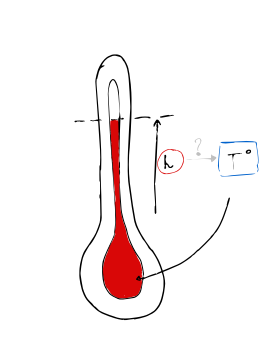
\includegraphics[clip, width=3cm]{Introduction/pics/therm_pb.png}     \\
    \caption{Thermometer Calibration}
    \label{fig:therm_calib}
\end{figure}


When interested in knowing the temperature, we observe the level of a thermometer.
In order to do so, someone had to graduate the thermometer. 
This seemingly simple action is rooted in a two-step process, which involves the construction of a theoretical model and its calibration using real-world data.

The first step involves accumulating theories and assumptions to construct a model linking the observed level and the actual temperature.
For instance, based on our knowledge of fluid dilation in response to temperature, assuming the diameter of the tube is constant with height, we can posit that the level is linearly correlated with the temperature.
This model introduces two parameters: the slope and offset of our linear model that need to be ascertained.

The second step involves determining these parameters. This step requires some calibration data as inputs. They are traditionally obtained by immersing the thermometer in icing and boiling water to acquire the levels corresponding to 0°C and 100°C.
  Using those data points, a linear system can then be used to solve for the parameters. Which finally gives use our level-to-temperature mapping


The solution, therefore, is a product of both theory and data, and can be reduced to two key components: the model and the algorithm. It demonstrates the importance of balancing abstract concepts with grounded data, and highlights how these two components interplay to produce tools for understanding and interacting with our world.

Interestingly, the model's complexity can often be inversely proportional to the amount of data required. For instance, a model with fewer assumptions demands more data. If we were to abandon the assumption of the thermometer tube's constant diameter, we would need to incorporate a parameterization of the tube diameter in our model. This addition creates more parameters and consequently demands additional data for calibration.

Conversely, having access to more data can allow us to work with fewer assumptions. Suppose we possess a well-calibrated thermometer that can provide unlimited data points. In that case, we could reduce our assumptions to a minimum and rely heavily on empirical evidence, marking each thermometer graduation using data directly from our well-calibrated thermometer.

Lastly, stronger assumptions demand less data. If we introduce the knowledge that the thermometer is immersed in boiling water, our mapping simplifies to a constant function, returning 100°C by convention and removing completely the need for data

With these carefully calibrated graduations now etched onto our thermometer, we can use the liquid level as a convenient stand-in for the temperature. However, an important question remains: How can we verify the accuracy of our newly calibrated thermometer?
% A few notes on this example:
% \begin{itemize}
% \item The first step takes in theoretical knowledge and uses a model to output candidate solutions
% \item The second step takes in data and uses an algorithm to output the solution
% \item The solution rely on theory and data and can be reduced to two components model and algorithm.
% \item Fewer assumptions in the model requires more data: If we loosen the assumption about the tube's constant diameter, we need to incorporate a parameterization of the tube diameter into the model, adding more parameters and necessitating additional data for calibration;
% \item More data requires fewer assumptions:If we have a well calibrated thermometer that provides us as many data as we want, we could make very little assumptions and just mark each graduation using data from the calibrated thermometer.
% \item Stronger assumptions requires less data: By adding the knowledge that the thermometer is in boiling water, our mapping is reduced to a constant function returning 100°C by convention.
%   \end{itemize}

% We now have graduations on our thermometer and can use the level as a proxy for the temperature without further thought!... Although how do we know if our calibrated thermometer is any good ? 
\begin{figure}[h]
\centering
\begin{tabular}{ccc}

    Step 1: 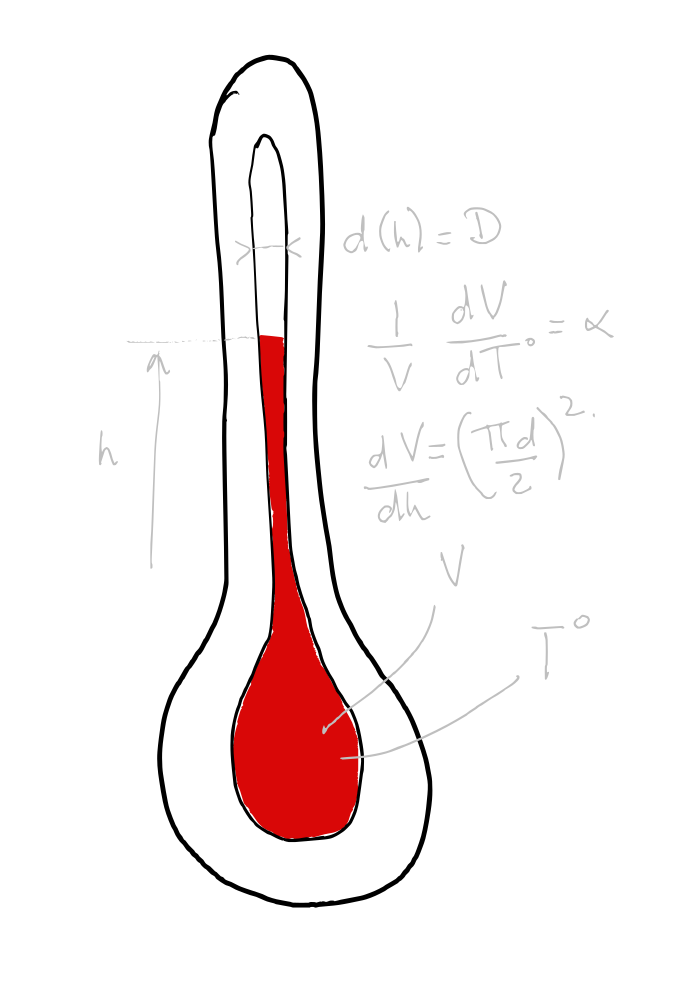
\includegraphics[clip, width=3cm, width=3cm]{Introduction/pics/therm_theroy.png} &    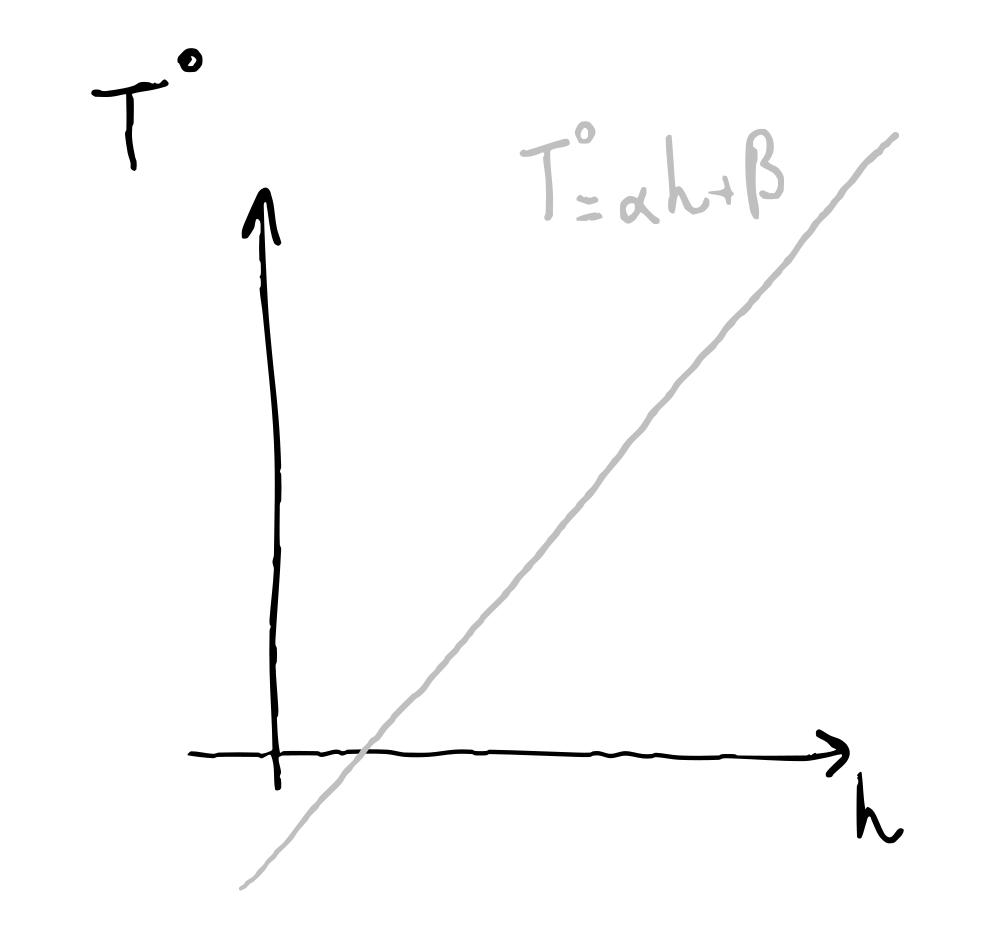
\includegraphics[clip, width=5cm]{Introduction/pics/therm_model.png}     \\  
     Step 2: 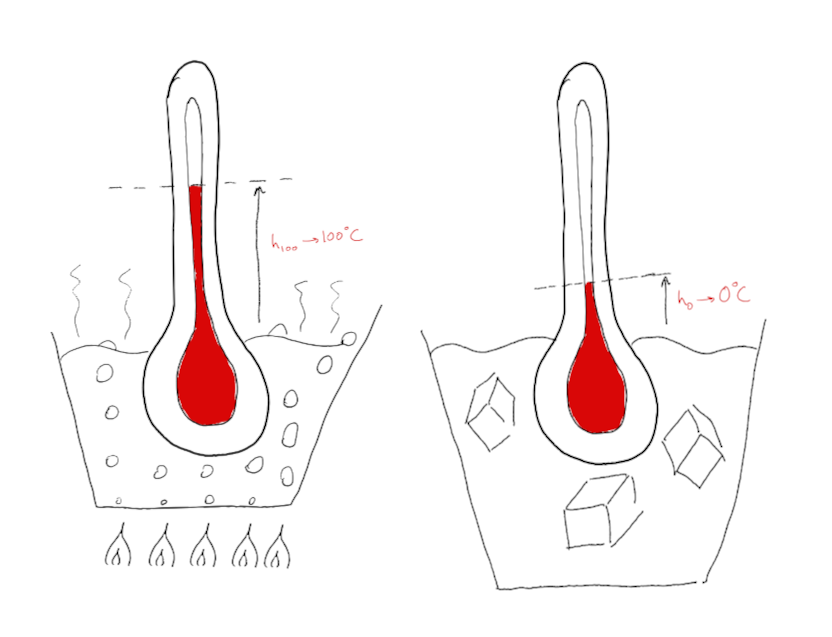
\includegraphics[clip, width=4cm, height=4cm, trim={2cm 1cm 2cm 2cm}]{Introduction/pics/therm_obs.png} &    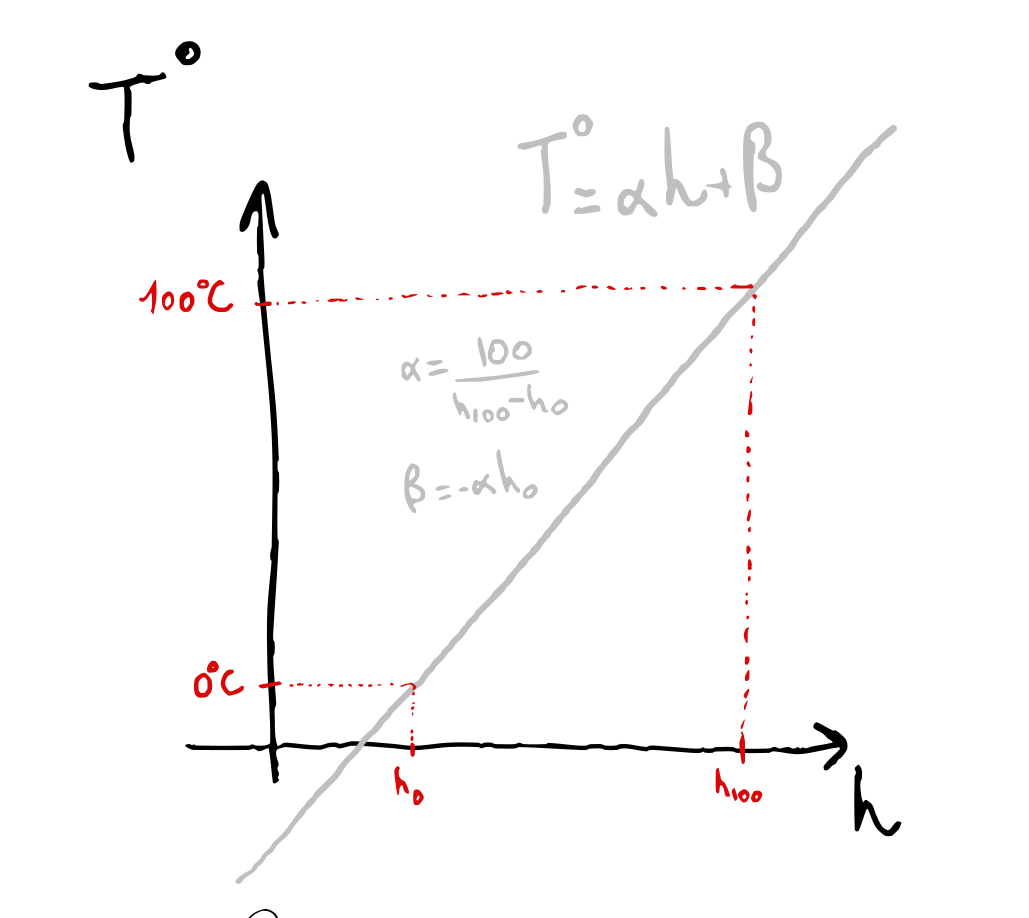
\includegraphics[clip, width=5cm]{Introduction/pics/therm_calib.png}     \\  
\end{tabular}

    \caption{Mapping thermometer level to temperature}
    \label{fig:therm_mapping}
\end{figure}

\subsection{Evaluation}

Without evaluation the use of our calibrated instrument would solely rely in the faith given to our mapping above.
Being novice calibrators we need to quantify the thermometers quality through metrics.

In our case the most intuitive metric for characterizing our thermometer's quality would be the precision of the temperature it gives.
Note that some situations may put importance on other characteristic such at the range at which it's functional.
  In order to properly evaluate our calibrated instrument, we need to test it in conditions corresponding to its intended use. (testing it domestic thermometer 5000 meter underwater is not not helpful).

 To do so, let's explicit some silent assumptions made on what we expect from our thermometer.
  For example that it needs to "be accurate to the half of degree", "have response time under 10 minutes", "work between -30°C and 200°C" "work at a reasonable atmospheric pressure" etc...

Then we need data to measure the precision of our thermometer in a way that is representative of how we want our thermometer to behave. Using a trustworthy reference like a third-party well-calibrated thermometer, we could compare the measurements of the reference with the one given by our solution.
  An example evaluation procedure could be to confront the measurements of the two instruments at different temperatures such as: in a freezer, in a fridge, at ambiant room temperature and in an oven.

Using the procedure above, we can now compute our metrics and assess if the quality of our calibrated thermometer.
This exercise, however, raises some critical points about evaluation. The process relies on two components that require a deep understanding of the thermometer's intended use: a suitable choice of metric and representative data. If the chosen metrics don't align with the intended use of the thermometer, the evaluation will be flawed. Similarly, if the data isn't representative of the thermometer's intended use, the evaluation will also be flawed.
 Furthermore, the reliability of the reference thermometer is pivotal. If the reference thermometer is not well-calibrated, the best of metrics won't be able to correctly evaluate our thermometer. 

It's also crucial to differentiate between calibration data, which is used to generate a solution, and evaluation data, which is used to assess the solution's quality.
A well-functioning thermometer should provide accurate temperature readings even for levels it wasn't calibrated on. Also, evaluation data should differ from calibration data. If we only measure precision at 0°C and 100°C, a thermometer that perfectly fits the calibration data would receive the highest metric, even if the other graduations are nonsensical.


% Some remarks about the evaluation:
% \begin{itemize}
% \item Evaluation rely on two components, a choice of metric and data
% \item If the metrics' choice are not suited to the intended use of the instrument, the evaluation will be flawed.
% \item If the evaluation data are not representative of the intended use of the instrument, the evaluation will be flawed.
% \item Defining relevant metrics requires intimate knowledge of the intended goal of the instrument.
% \item If the reference thermometer is biased (not well calibrated) a good metric will not define a thermometer of quality
% \item Evaluation and calibration data have different purposes: calibration data is used to give a solution, evaluation data is used to assess the quality of a solution
% \item A good thermometer should give correct temperatures even for levels it were not calibrated on.
% \item Evaluation data should be different than calibration data: If the evaluation only measured the precision at 0°C and 100°C, fitting the calibration data would get the highest metric even if all other graduations were non-sense.
% \item Different metric can produce different rankings, therefore the evaluation is relative to the metric choice
% \item An evaluation can use multiple metrics, therefore no ranking between two methods is guaranteed
% \item Both the single accuracy in the oven and the mean or standard deviations of the different measured accuracies can be considered as metrics
% \end{itemize}


 \subsection{Sources of errors}

Given an evaluation procedure, the errors are the gap to the reference and can be attributed to three sources.

\begin{figure}
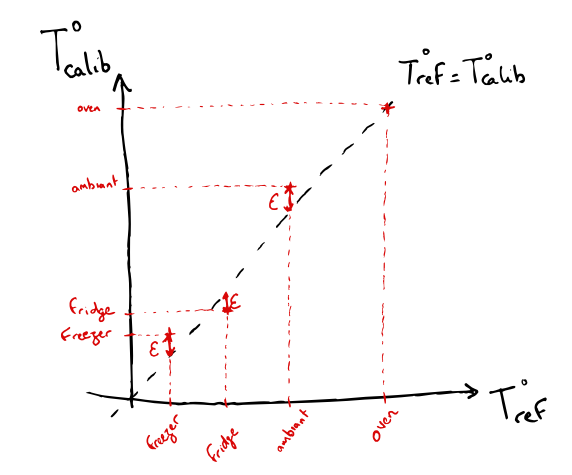
\includegraphics[clip, width=6cm]{Introduction/pics/errors.png}  
\begin{tabular}{c |c|c}

     \hspace{-.15\linewidth}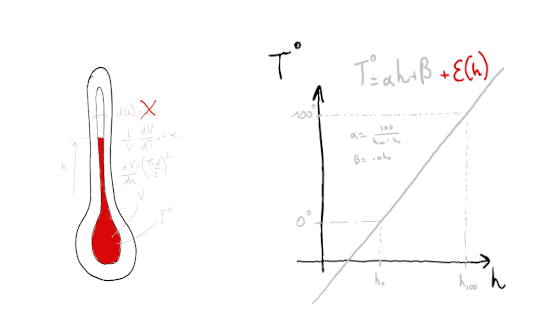
\includegraphics[width=.4\linewidth]{Introduction/pics/model_err_w_source.png}  &
     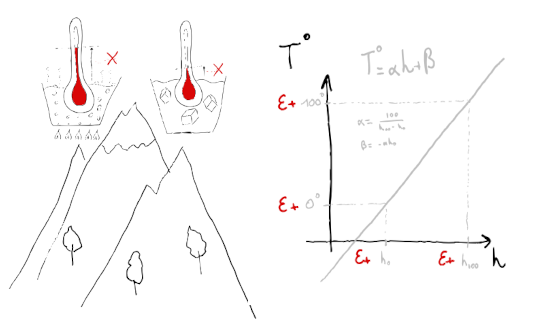
\includegraphics[width=.4\linewidth]{Introduction/pics/data_err_w_source.png} &
     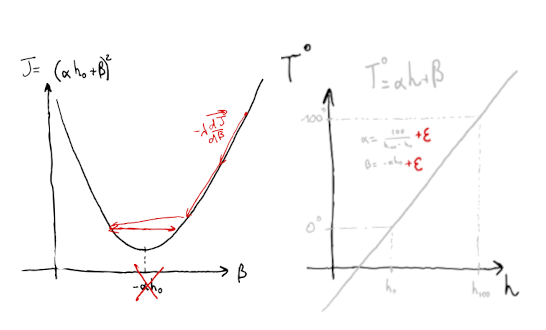
\includegraphics[width=.4\linewidth]{Introduction/pics/optim_err_w_source.png} \\
     \hspace{-.15\linewidth}Model &  Data &  Algorithm \\
\end{tabular}
    \centering
    \caption{Sources of errors}
    \label{fig:err_sources}
\end{figure}
 The model is a source of error if the assumptions made were inaccurate. For example if the diameter of the tube is not constant with height the linear correlation between level and temperature is not exact and will induce errors when interpreting the level.

 Even with perfect assumptions, noisy data can introduce errors in the calibration. If we interpreted our 0°C and 100°C in icing and boiling water at the top of a mountain with lower atmospheric pressure, we will have calibrated our parameters with erroneous measurements and the subsequent graduation of our thermometer will be inaccurate.

 Finally even with perfect assumption and perfect data, the algorithm used to find the solution's parameters can be a source of errors if it fails to find the optimal parameters. For example if we solve for the parameters with a gradient descent method, using a step size too big will prevent finding the exact parameters which will also generate errors in the subsequent measurements.

In order to develop a calibration procedure, we need to take those sources of error into account. The calibration procedure choice will not only depend on the level-temperature relationship but on the whole relationship between calibration data to the final calibrated thermometer. We therefore need to incorporate in our reasoning the how the calibration data was acquired, what is the best model to map the level to the temperature, and what is the best algorithm to find the optimal parameters of the model.

This leads us to the following problem "How to find the best thermometer calibration procedure?"

\subsection{Finding the best thermometer calibration procedure}
In the process of finding a solution to the level-temperature mapping problem, we need to define a model, an algorithm, and have access to calibration data. Additionally, to evaluate our solution, we need to define a metric and have access to evaluation data. Interestingly, these components can be specified at a higher level for solving and evaluating the calibration procedure itself, essentially creating a meta-level or "second order" problem.

The \textbf{Model}, in this second order scenario, combines different assumptions to determine the set of potential calibration procedures. This model defines the space in which the calibration procedures exist and interact based on a set of assumptions about what makes a good calibration procedure.

The \textbf{Algorithm} is used to select the best calibration procedure. This could be as straightforward as testing different combinations and choosing the most effective one, or it could involve complex numerical optimization procedures to determine higher-level parameters.

The \textbf{Calibration Data}, at the second order, consists of calibration tasks with a method to assess the performance of candidate procedures. This allows the algorithm to select the best solution.

The \textbf{Evaluation Metric} should reflect the intended use of the calibration procedure, including the range of thermometer calibrations we plan to use this procedure for. A useful metric might be the precision of all the thermometers we aim to calibrate using the proposed solution.

The \textbf{Evaluation Data} should be representative of the variety of intended uses. This means it should contain calibration tasks for a range of thermometers of interest. Additionally, we need a reference for these tasks to measure the precision of our solution.

By leveraging these five components, we can select the best calibration procedure, quantify its quality using the evaluation data, and use it to calibrate new thermometers with confidence in the resulting calibrated instrument. This parallels the problems of "Finding the level-temperature mapping" (which we refer to as the first order problem) and "Finding the calibration procedure" (the second order problem) and offers insights for further research in this field.

Note that second order metrics can extend beyond the scope of the first order problem. These metrics could encompass aspects such as robustness to noise or the computational complexity of the calibration procedure. This means our evaluation of a calibration procedure not only includes how well it measures temperature, but also how well it handles uncertainties or computational burdens.

A second order solution can be conceptualized as a function. This function would accept first order calibration data as inputs, which contain the properties and measures of a specific thermometer and their corresponding responses. The output of this function would then be a first order solution - a tailored calibration procedure for the thermometer represented in the data.

The second order problem also involves making decisions on parameters to select the best solution, which can take various forms. For instance, these parameters can be discrete choices between different assumptions, like whether to consider the thermometer's tube diameter as constant or not. These decisions shape the model at a high level and can fundamentally alter the characteristics of the calibration procedure. The parameters can also denote choices between different first order algorithms like choosing a direct linear system inversion or a iterative optimization procedure. Lastly, these second order parameters can be constants in the level-temperature mappings or parameters of an optimization procedure, like step size. This shows that the parameters in the second order problem have a broad range of applicability, affecting both the details of the calibration procedure and how the procedure is chosen.


Finally, a critical note is that the data used to evaluate a solution at the second order level should still be separate from the training data. This principle holds true for the same reasons it applies to the first order problem - using distinct data sets helps to ensure that our solutions generalize well beyond the specific scenarios they were trained on.

\section{From thermometer calibration to generic observation problems}
\subsection{Introducing time}
Our previous example focused on the static calibration of a thermometer. However, in the real world, temperature measurement is often a dynamic process. The response time of the thermometer —the duration required for the indicated level to reflect the accurate temperature of its location — becomes a critical factor.

This dynamic scenario introduces a more complex case where we infer the temperature, our quantity of interest, from a series of observations over time. This shift has implications for the components of our method.

For instance, the evaluation metrics must now consider the dynamical characteristics of the thermometer calibration. The model must account for additional factors, including assumptions about how temperature diffuses over time. Similarly, the algorithm used to select the best solution must adapt to these changes.

In this dynamic context, we have the choice of considering the dynamic aspect as a separate or join problem to the calibration. We could treat the thermometer's level readings as direct observations or infer the dynamic temperature from the already calibrated thermometer's recent observations. These choices impact our assumptions about the model and the noise in the data.

\subsection{Introducing space}
Until now, we have focused on measuring temperature at a single location. However, in many cases, we may need to understand the temperature field across a spatio-temporal domain—a much more complex problem.

We can formulate this problem hierarchy as follows:

\begin{itemize}
    \item First-order problem: Determine the temperature field in a room over a specific period, given observations from thermometers located at different places and times.
    \item Second-order problem: Develop a procedure that maps a set of observations to the temperature field.
\end{itemize}
    
    

Just as we did in the static and dynamic cases, we apply our conceptual blocks—evaluation metrics, modeling, algorithm selection, and data consideration—in this spatio-temporal context. This approach allows us to handle the added complexity while remaining grounded in our fundamental methodological framework.

\subsection{The case of satellite altimetry}
  The thermometer provided a good stepping stone to introduce the necessary concepts.
  However the actual problem we're interested in is to estimate the sea surface height (SSH) on the surface of the ocean given satellite data.
The process of calibrating a thermometer, as previously illustrated, shares a fundamental conceptual parallel with the task of estimating sea surface height (SSH) using satellite data. Just as we use a thermometer to measure temperature by observing the liquid level, satellite altimetry allows us to estimate the SSH by interpreting specific signals and measurements from a much larger and more complex system.

In both cases, we observe certain behaviors or conditions—be it the level of liquid in a thermometer or the satellite observations of the ocean surface—and use these to infer something about the underlying state of the system we are interested in. Both rely on the creation of a model based on existing knowledge and assumptions, and then fine-tuning that model using calibration data to map observed behavior to the desired quantity.

The temporal aspect is also shared. Much like the response time of a thermometer, which determines how quickly it can accurately measure the temperature of its environment, satellite data gives us a series of snapshots over time from which we can reconstruct the dynamic behavior of the sea surface.

When considering the spatial dimension, estimating SSH is like placing thermometers across a room to understand the distribution of temperature in that space. The same principle is applied to satellite altimetry, but on a much larger scale, mapping the Earth's oceans.

In essence, both cases involve observing a system, interpreting those observations through a theoretical model, and refining that model with real-world data to give us the most accurate understanding possible. The application and scale are vastly different, but the underlying principles of observation, modeling, calibration, and evaluation are consistent.

  Furthermore satellite altimetry which gives us information on the sea surface height (SSH) offers a compelling case study.
  The SSH is related to surface dynamics and current operational products do not resolve processes below 150 km, which are essential for climate monitoring.
  This situation underscores a significant gap in our observational capabilities.
  The recent deployment of a novel sensor during the SWOT satellite mission provides numerous opportunities to address this gap.
  This new sensor introduces unprecedented calibration challenges due to previously unseen errors, but it also promises to enhance the reconstruction of SSH maps.
This manuscript, therefore, aims to explore the application of deep learning to two key observation problems related to these issues. The first is estimating SSH from noisy SWOT observations, and the second is inferring the complete SSH field from partial measurements.
  
  As such the contributions of this manuscript explore the application of deep learning to these two observations problems: estimating the SSH from the noisy SWOT observations and estimating the complete SSH field from partial measurements.
  This allows us to formulate the two problems that will be addressed in the manuscript.
  \begin{itemize}
      \item Given scarce calibrated altimetry observations and uncalibrated SWOT observations, estimate the SSH on the domain observed by SWOT
      \item Given scarce SSH observations, estimate the SSH on the whole domain considered
  \end{itemize}
  \begin{figure}
      \centering
          \begin{tabular}{c|c}
            \hspace{-0.2\linewidth}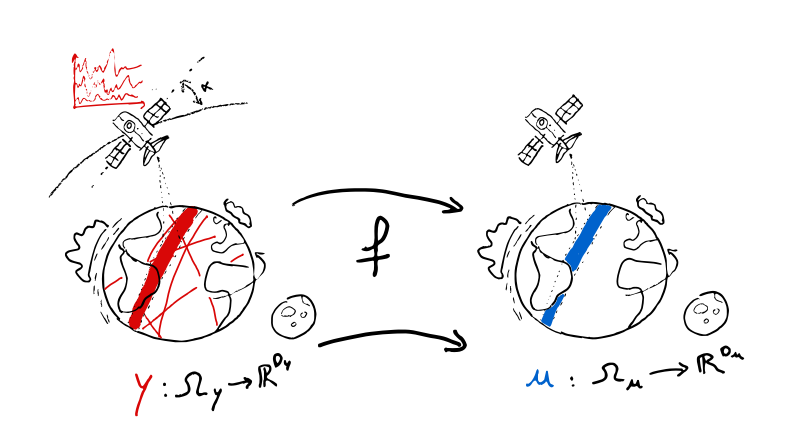
\includegraphics[width=0.7\linewidth]{Introduction/pics/calib_task.png}   & 
            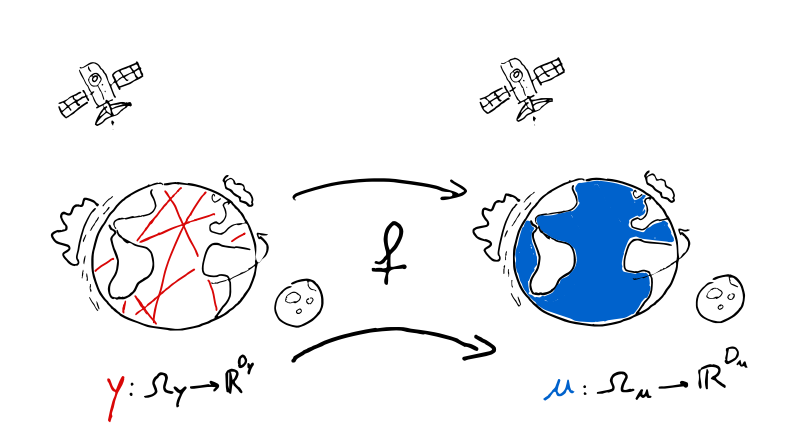
\includegraphics[width=0.7\linewidth]{Introduction/pics/mapping_task.png}\\
           \hspace{-0.2\linewidth} SWOT calibration task & Nadir Altimetry mapping task \\
          \end{tabular}
      \caption{Altimetry observation problems}
      \label{fig:altimetry task}
  \end{figure}

\section{Deep learning potential for altimetry problems}
\subsection{Existing approaches: Model driven versus data driven}

Looking back at remarks of the problem of level-to-thermometer mapping. We noted the feedback loop between model and data.
Under the assumptions that the diameter is constant model of the thermometer, we need two datapoints, If I relax the assumption about the constant diameter and fetch additional data to calibration the new parameters.
On the other hand data driven approaches first frame the problem as an interpolation task and will chose the assumptions that fit the data available.
Given two data points, a reasonable set of candidates to search is the set of linear functions. Given a thousand data points, I can model the mapping with a nearest interpolator effectively reducing my assumptions to stationary (the same level will give the same temperature) and smoothness (the temperature will be close between two levels close by)

Model driven: The strongest assumptions we have the less data we need. The weakest assumptions we have the more data we need.
Data driven: The best data we have, the less assumptions we need. The worst data we have, the more assumptions we need.

\subsection{Deep learning for computer vision and natural language}
Deep learning brings forth models, such as neural networks, that are predicated on very weak assumptions. Their strength lies in the fact that, given their sufficient width, they can approximate any function. This leads to deep learning models defining vast sets of potential candidates, consequently requiring substantial datasets and sophisticated algorithms to find the best fit.

Innovations in model architectures such as ResNet, batch normalization, and in optimization procedures like Stochastic Gradient Descent (SGD), Adam, and various learning rate schedules have consistently improved the search of larger spaces for candidate solutions, therefore  enabling the use of larger neural networks. 
However, the fact that deep learning models can in theory approximate any function introduces a peculiar consideration which is that fitting exactly the calibration data gives you no guarantee on how the model will behave on unseen data. The gap of performance between "seen" and "unseen" data is called the generalization gap. This has standardized the practice of splitting the calibration data in two sets: training and validation. The training set is used  by the optimization procedure to search for the parameters whereas the validation set is used to assess the quality of each candidate. 
Addressing the problem of generalization have motivated many innovations in regularization, architectures, initialization schemes and data augmentation techniques.


When looking at different application domain, the track records of deep learning in computer vision and natural language are especially impressive. 
The combination of models and algorithm brought by deep learning have managed to solve tasks that previously unsolved.
This can be intuitively understood when considering the challenges of a binary classification task between cats and dogs.
Precisely that the mapping between natural images to binary label is quite difficult to explicitly formalize using domain knowledge. 
The task of predicting the next word of a sentence as done by current LLMs is similarly challenging to model using linguistic theory.

Presented as such deep learning seems to provide universal tools,  
however we would like to stress two factors that seem of great importance when looking at the contributions of deep learning in specific fields.
The first factor is quality and availability of data, indeed the creation of large, curated datasets, like ImageNet in computer vision or ThePile in natural language processing have shown to dramatically expedite the development of novel approaches. 
The second factor is the design of informed architectural patterns that are particularly suited to the domain, leading to performance breakthroughs. Examples of these include convolution techniques and U-Net architectures in computer vision, attention mechanisms in natural language processing.


Compared to other application domain such as CV and NLP, observation problems present a different context for applying deep learning. 
On one hand quite extensive theoretical knowledge have been accumulated on the dynamics that gives structure to the data and that explicitly links the observations with the quantities of interests.  
On the other hand the available data made of observations and numerical model outputs, although consequent, presents challenges since we never have access to the ground truth quantity we want to estimate. (The best we can do is consider a calibrated instrument as ground truth when it's observed). 



This adds
Given a problem stated as above, deep learning brings to the table its set of tools for defining candidate solutions to a problem as well as optimization procedures for searching this set for the optimal candidate.

The main 
Deep learning research keeps demonstrating its potential in exploiting complex structures from data outperforming model driven approaches.
This has been blatant in computer vision over the last decades and in natural language processing over the last years.
Although the progress of deep learning as a generic tool is undeniable when looking at the ever wider range of tasks its applied to.

This manuscript will specifically address these two facets — comprehensive, well-curated datasets and efficient architectural patterns — of deep learning when applied to observation exploitation.

Computer vision and NLP are probably fertile ground for deep learning due to the difficulty of defining models that capture the complex nature of natural language or natural images and that large datasets were accumulated in those fields. 



This constitutes an interesting setup for synergizing physical priors and deep learning models.

Given the 

% \subsection{Model driven, Data driven}
% Looking back at remarks of the problem of level-to-thermometer mapping. We saw the feedback loop between model and data.
% We designate model driven, approaches that first frame the problem as a modelling task and then use the data that fits the assumptions they make of the system.
% Under the assumptions that the diameter is constant model of the thermometer, we need two datapoints, If I relax the assumption about the constant diameter and fetch additional data to calibration the new parameters.
% On the other hand data driven approaches first frame the problem as an interpolation task and will chose the assumptions that fit the data available.
% Given two data points, a reasonable set of candidates to search is the set of linear functions. Given a thousand data points, I can model the mapping with a nearest interpolator effectively reducing my assumptions to stationary (the same level will give the same temperature) and smoothness (the temperature will be close between two levels close by)

% Model driven: The strongest assumptions we have the less data we need. The weakest assumptions we have the more data we need.
% Data driven: The best data we have, the less assumptions we need. The worst data we have, the more assumptions we need.


\subsection{contributions}
More precisely we'll ask wether deep learning can help better exploit satellite observations for improving our knowledge of sea surface dynamics.


Deep learning and earth observation are two well established fields with accumulated knowledge, conventions, and best practices. 
This introduce challenges when developing transdisciplinary approaches that aim to combine expertise from the two fields.
Interfaces need to be proposed to this end which will serve as bridge for domain experts to explore the other side.
Evaluation and data from ocean scientists to ML practicioners. 
Didactic, Generic purpose, and modular implementation of a neural data assimation algorithm for addressing a range of observation problems from ML to ocean



\end{bibunit}

